\def\QRCODE{MASTER_mispa_TUT.IMG.colip_matlabqrcode.png}
\def\QRPAGE{http://www.iptutorials.science/tree/master/MASTER_mispa/TUT.IMG.colip/matlab}
\mcorrectionsection{Matlab correction}


The maximal value is $M_0$, arbitrarily fixed at 100.

\begin{matlab}function M0 = getColipM0()
% return M0 value
M0 = 100;
\end{matlab}

\subsection{LMS tones}
This is the difficult part of LIP and CoLIP. Be careful with the use of the function \minline{eps} that returns the precision at a given double value.
\begin{matlab}
function [ lms ] = lmstone( LMS )
% convert LMS values to color tones
% each LMS channel is normalized
M0 = getColipM0();
lms = (M0-eps(M0))*(1-LMS/M0);  
\end{matlab}

\subsection{Isomorphism}
The isomorphism is the conversion into/back from the logarithmic space.
\begin{matlab}
function x = phi(f, M0)
% LIP isomorphism 
% f : graytone function 
% M0: maximal value
x = -M0*log(1-f/M0);
\end{matlab}

\begin{matlab}
function f = invphi(x, M0)
% inverse isomorphism
f = M0 * (1-exp(-x/M0)
\end{matlab}

\subsection{XYZ to LMS}
\begin{matlab}
%% convert from XYZ to LMS
% XYZ: data array of dimensions [m, n, 3]
% MatPassage: string 'hpe', 'hped64', 'bradford', 'ciecam02'

function LMS=XYZ2LMS(XYZ,MatPassage)
if ndims(XYZ) == 3
    s=3;
    [M,N]=size(XYZ(:,:,1)); 
    XYZ=reshape(XYZ,[M*N,3])';
else
    s=2;
end

switch (MatPassage)
    case('hpe')
    U=[0.38971, 0.68898, -0.07869; -0.22981, 1.18340, 0.04641; 0, 0, 1];
end  

% conversion
LMS=U*XYZ;
if s==3
    LMS=reshape(LMS',[M,N,3]);
end
\end{matlab}

\begin{matlab}
function XYZ=LMS2XYZ(LMS,MatPassage)
% convert from LMS into XYZ
% LMS: data array of dimensions [m, n, 3]
% MatPassage: string 'hpe', 'hped64', 'bradford', 'ciecam02'

[M,N]=size(LMS(:,:,1)); 
LMS=reshape(LMS,[M*N,3])';
switch (MatPassage)
    case('hpe')
    U=[0.38971, 0.68898, -0.07869; -0.22981, 1.18340, 0.04641; 0, 0, 1];
end

XYZ=U\LMS; % inv(U)*LMS
XYZ=reshape(XYZ',[M,N,3]);
\end{matlab}

\subsection{CMF}
The color matching functions are provided for convenience. There exist many resources on the internet where they can be found. The classical diagram in the xy space (the horseshoe) is shown in Fig.\ref{fig:colip:matlab:xy}.

\begin{matlab}
load 'cmf.mat'

xn = SpecXYZ(:,:,1)./sum(SpecXYZ, 3);
yn = SpecXYZ(:,:,2)./sum(SpecXYZ, 3);
zn = 1-xn-yn;

scatter(xn, yn, 30, cmap, 'filled');
\end{matlab}

\begin{figure}[htbp]
	\centering
	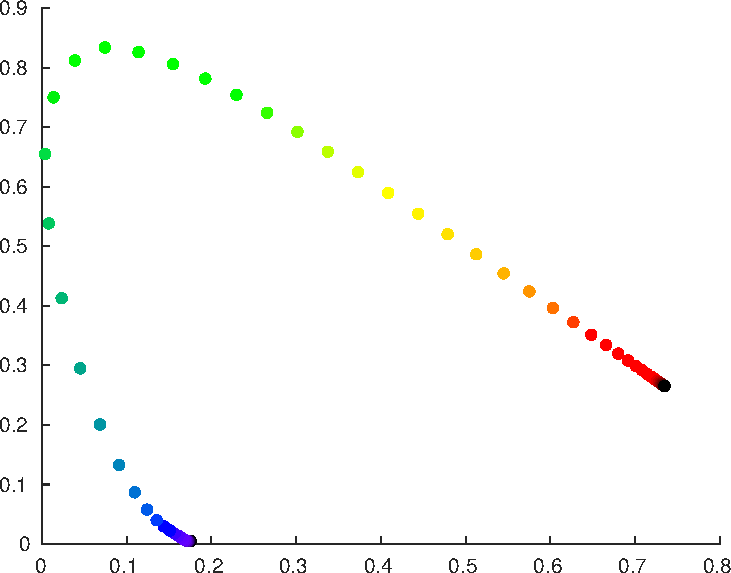
\includegraphics[width=.8\linewidth]{xy.pdf}
	\caption{Color matching functions in the xy space.}
	\label{fig:colip:matlab:xy}
\end{figure}

To display the CMF and the cube of all RGB colors in the  $(\h{rg},\h{yb})$ space, the following code is used:
\begin{matlab}
ARGYB_hat = LMStoARGYB_chapeau(SpecLMS);
figure(2),
hold on
scatter(ARGYB_hat(:,1,2), ARGYB_hat(:,1,3), 30, cmap, 'filled');

% purple line
purple_ARGYB_hat = LMStoARGYB_chapeau(pourpresLMS);
scatter(purple_ARGYB_hat(:,1,2), purple_ARGYB_hat(:,1,3), 30, 'black', 'filled');

% RGB cube
step=10;
[R, G, B] = ndgrid(0:step:255, 0:step:255, 0:step:255);

R = reshape(R, numel(R), 1);
G = reshape(G, numel(G), 1);
B = reshape(B, numel(B), 1);

cubeRGB = cat(2, R, G, B)/255;
cubeRGB = reshape(cubeRGB, size(cubeRGB, 1), 1, 3);
colCubeRGB = reshape(cubeRGB, size(cubeRGB,1), 3);

% conversion from RGB to a,rg,yb hat
cubeXYZ = rgb2xyz(cubeRGB, 'WhitePoint', 'e');
cubeLMS = xyz2lms(cubeXYZ, 'hpe');
cube_ARGYB_hat = LMStoARGYB_chapeau(cubeLMS);
% display result
scatter(cube_ARGYB_hat(:,1,2), cube_ARGYB_hat(:,1,3), 30, colCubeRGB, 'filled');
\end{matlab}

The results is shown in Fig.\ref{fig:colip:matlab:rgyb}. The following functions are used for the conversions.
\begin{matlab}
function ARGYB_chap=LMStoARGYB_chapeau(LMS)
% LMS: normalized values in ]0;M0]

ARGYBtilde = LMStoARGYBtilde(LMS);

% conversion
ARGYB_chap = ARGYBtildetoARGYBchap(ARGYBtilde);
\end{matlab}


\begin{matlab}
function ARGYBtilde = LMStoARGYBtilde(LMS)
%%%%%%%%%%%%%%%%%%%%%%%%%%%%%
% maximal values definition
M0 = getColipM0();
[m,n,~] = size(LMS); % image size

% conversion to (L~,M~,S~): applying LIP isomorphism
%warning('notice epsilon for conversion into lms tones')
LMSton = lmstone(LMS);
LMStilde = phi(LMSton, M0);

% conversion to antagonist color space (a~,rg~,yb~)
P = [40/61,20/61,1/61;1,-12/11,1/11;1/9,1/9,-2/9 ]; % antagonist matrix
LMStilde = reshape(LMStilde,[m*n,3]);
LMStilde = LMStilde';
ARGYBtilde = P*LMStilde;
ARGYBtilde = ARGYBtilde';
ARGYBtilde = reshape(ARGYBtilde,[m,n,3]); 
\end{matlab}

\begin{matlab}
function ARGYBchap = ARGYBtildetoARGYBchap(ARGYBtilde)
% function for conversion, takes absolute value
Max = getColipM0();

ARGYBchap(:,:,1) = invphi(ARGYBtilde(:,:,1), Max); 

for c=2:3
    tmp =  abs(ARGYBtilde(:,:,c));

    ARGYBchap(:,:,c) = sign(ARGYBtilde(:,:,c)) .* invphi(tmp, Max);
end

end
\end{matlab}


\begin{figure}[htbp]
	\centering
	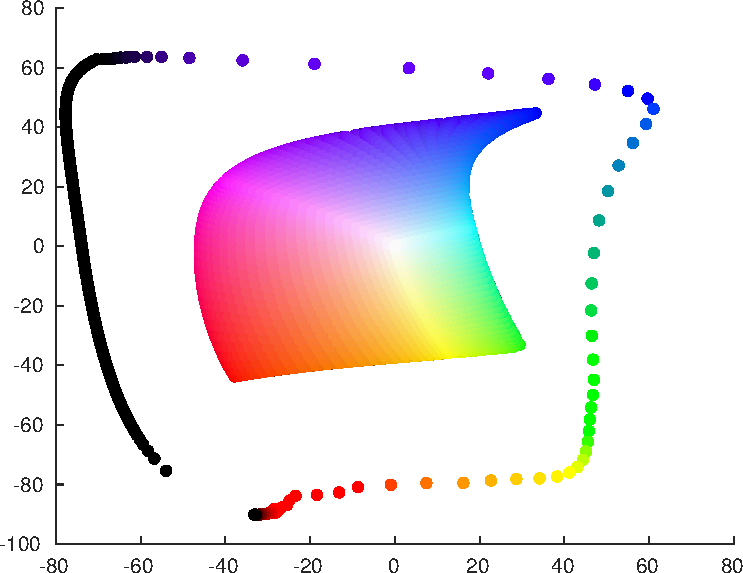
\includegraphics[width=.8\linewidth]{argyb.pdf}
	\caption{Color matching functions in the $(\h{rg},\h{yb})$ space.}
	\label{fig:colip:matlab:rgyb}
\end{figure}
